\chapter{Introduction}
\label{chap:1}
\ChapterPageStuff{1}

\section{Preamble}
Maintenance of software systems is continuous and is a reduced form of software
development \cite{Sneed2004}.~Software maintenance needs to be done on regular
systematically procedure in its entire lifespan. Most companies will strife to increase their digital products and services over the life cycle of the software project \cite{Niu2018},\cite{Galster2019}.

\section{Background}
Software maintenance is an essential task in software development as it can directly reduce cost and effort to create new software systems \cite{FrancisThamburaj2017}. According to a study of the total development cost for a typical software maintenance efforts, conducted by the United States Department of Commerce found that the cost can be as much as $60\%$-$80\%$ of the total cost of the software systems entire development life cycle \cite{Ogheneovo2014}. These costs will increase to maintain much older and more complexed software systems, therefore it is key to the feasibility of the software systems to implement maintenance on it~\cite{Alenezi2016}.\par Under most circumstances maintenance is implemented if a software system does not meet the required functions specified by the performance requirements \cite{Ogheneovo2014},\cite{Sneed2004}.

\begin{figure}[!htb] % An h :here, t: top, b: bottom.
    \centering % cent the figure
    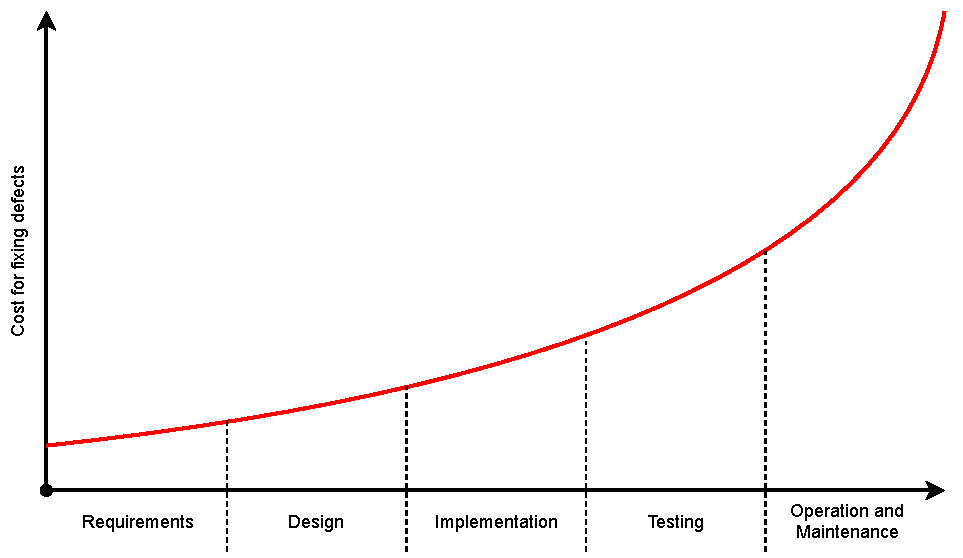
\includegraphics[width=0.6\textwidth]{Images/Chapter1/Background/Cost_of_fixing_bugs/Cost_of_fixing_bugs.pdf}
    \caption{Facial recognition Process}\label{fig:facial recognition process}
\end{figure} 

\newpage

\subsection{Need for a logging mechanism}
No study was found where both the logging mechanism and analysis were combined.
There is a need to develop a method to implement a user-activity logging
the mechanism to do further analysis of the logs to improve software
maintenance.

\subsection{Objectives of the study}
The goal of the study is to develop a logging mechanism to track user-based
activities to preform analysis of these logs to improve system maintenance in
software environment. The study is divided in two components to achieve the
primary goal which is the design and implementation of the logging mechanism
and the analysis of the system utilisation to improve system maintenance.

\subsubsection{Logging mechanism:}
\begin{itemize}
    \item Random text.
\end{itemize}

\subsubsection{Analysis of the system utilisation to improve software maintenance}
\begin{itemize}
    \item Random text.
\end{itemize}

\subsection{Overview of the dissertation}
\subsubsection{Chapter 1: Introduction}
This chapter contains the background of software maintenance and system
utilisation analysis.
\subsubsection{Chapter 2: Mehtodolgy}

\newpage
\section{Literature Study}

\subsection{Preamble}
Introduction of section.

\subsection{Software Maintenance}

\subsection{Event-based logging}
In this section the event-based logging will be discussed and how it is part of software maintenance. 

\subsection{User-based activities in Web-based applications}
In this section, the user-activities in Web-based applications will be discussed.

\subsection{Logging mechanism development}

\section{Conclusion}

